\chapter{Complex variables and vector spaces}
\minitoc
\pagebreak
\section{Complex Numbers revision \& mappings}
\subsection{Basics}
We start with a basic revision of complex numbers.
 Complex numbers were initially introduced to ensure that every polynomial of degree n has n roots. 
 A complex number, $z$, can be expressed in 3 forms:
%
\begin{enumerate}
	\item $z=x+iy$
	\item $z=R(cos\theta+isin\theta)$
	\item $z=Re^{i\theta}$
\end{enumerate}
%
In case your memory is poor, $i$ is the square root of -1.
 Addition of complex numbers is defined as follows,
 $$ (x+iy) + (a+ib) = (x+a) + i(y+b), $$
 which should be obvious.
 Subtraction is not explicitly defined, but is easy to understand by changing $a$ to $-a$ and $b$ to $-b$.
 Multiplication is also defined as
 $$(x+iy)(a+ib) = (ax-by)+i(bx+ay).$$
%
\subsection{Argand Diagrams}
An Argand diagram is a way of representing a complex number on a 2D plane.
 The real component of $z$ is plotted on the x-axis whilst the imaginary component is plotted on the y-axis.
%
\begin{minipage}[t]{0.47\linewidth}
	\begin{figure}[H]
 		\centering
 		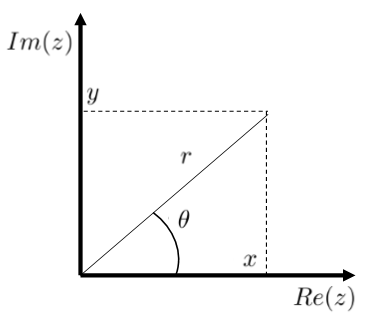
\includegraphics[width=\linewidth]{complex/argand}
 		\captionsetup{font=small} 	
	\end{figure} 
\end{minipage}
\hspace{0.6cm}
%
\begin{minipage}[t]{0.47\linewidth}\(\)
	\vspace{1cm}
	We can define the modulus, 
	%
	\begin{align*}
		|z| &= \sqrt{x^2+y^2} \\
		&= (x+iy)(x-iy) \\
		&= z\overline{z}.
	\end{align*}
	%
	In addition to this, $\theta$ is often referred to as the argument.
	 Note that the argument is not unique; you can add $2\pi$ to the argument and obtain the same result, so it is often useful to think of the principal value argument adding the contraint that $\theta$ lies between $0$ and $2\pi$
\end{minipage}
%
\begin{examples}
	We begin with a few basic examples to refresh your memory, given $z_1=1+i$ \& $z_2=2+3i$:
	\begin{enumerate}
		\item Find the cube root of $z_1$
		\item Find the modulus and argument of $z_1z_2$
	\end{enumerate}
\textbf{Answers:} 1. $2^{1/6}exp(\frac{\pi}{12})$, $2^{1/6}exp(\frac{3\pi}{4})$, $2^{1/6}exp(\frac{17\pi}{12})$ \hspace{0.5cm}
2. $|z| = \sqrt{26}$, $arg(z)=1.77$
\end{examples}
%
\subsection{Functions and Mappings}
Here we take a slightly abstract and brief detour to discuss functions.
 Up until slightly over a century ago a mathematician's view of a function was probably very similar to what the reader has now.
 Usually it is a formula that takes in values of a variable, say $x$, and outputs another number, $f(x)$.
 However, it became clear that this very restrictive definition of a function would not suffice in the modern world, so we needed a more abstract definition.
 The reader may be familiar with this more abstract definition, without realising it, if they've done any computer programming.
 For example, in \textbf{Python} you may want to make a function that takes in inputs from the user of `yes' or `no', and outputs `1' if the user inputs `yes' or a `0' if the user inputs `no'.
 There are many ways of visualising what a function does, the reader will probably be familiar with a graphical interpretation.
 Alternatively, a more abstract function can be viewed as a mapping. 
\par     
We need to define the \emph{domain}, D and \emph{co-domain} (or range), R of a function with the former corresponding to all the values that can be input to the function, and the latter corresponding to all outputs of the function.
 The most useful way to think about this is in terms of sets: a function takes vales from a set, D, and assigns each value in D a corresponding value in R.
 For example in our programming analogy we take the domain as \{`yes',`no'\} and the range as \{`1',`0'\}. 
 Anyone making this kind of function will know that they will have to restrict the user's inputs to just `yes' or `no', either by only displaying 2 buttons, or by including an error message and loop if the user inputs something unexpected.
 This is because the domain of this function is \{`yes',`no'\} so this function can only accept the values `yes' and `no'.
\par 
This more abstract definition of a function can be used to understand functions of a complex variable.
 We can consider the function $f(z)$ as a mapping, taking the values from the complex plane, Z, to another complex plane, W.
 Every complex number in the domain of the function will have a corresponding value in the range. However now we would need 4 dimensions to present this as a graph like we do for functions of one variable, so it's easier to visualise as changing from one plane to another.
 For example, consider $w=z^2$, what does this mapping look like?
 If we assume $w=X(x,y)+iY(x,y)$ we can see that $X=x^2-y^2$ \& $Y=2xy$.
%
\begin{minipage}[t]{0.47\linewidth}
	\begin{figure}[H]
		\centering
		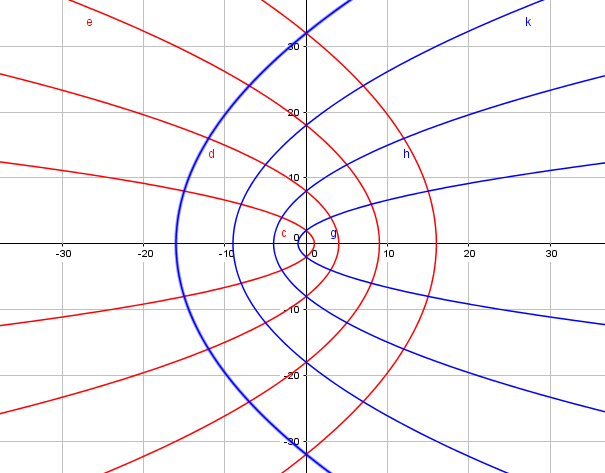
\includegraphics[width=\linewidth]{complex/mapping}
		\captionsetup{font=small} 	
	\end{figure} 
\end{minipage}
\hspace{0.6cm}
%
\begin{minipage}[t]{0.47\linewidth}
	\vspace{0.3cm}
	With a little bit of magic algebra, by setting $x=a$ and $y=b$ we can get 2 relationships.
	\begin{align*}
	\frac{Y^2}{4a^2}=a^2-X \\
	\frac{Y^2}{4b^2}=X+b^2. \\
	\end{align*}
These 2 equations [and you should check these] are plotted on the left for different values of $a$ and $b$.
 Remembering that $a$ and $b$ are $x$ and $y$ respectively, the red lines are how lines of constant x in the z-plane map into the w-plane.
\end{minipage}
%
%
\subsection{The argument theorem}
Consider a function $f(z)$, if $f(z_1)=0$ then $z_1$ will map onto the point $w=0$ in the w-plane.
 The argument theorem states that if a contour in the z-plane wraps around $n$ roots of $f(z)$ then it's mapping will wrap around $w=0$ $n$ times. 
 This is illustrated below:
\begin{figure}[H]
	\centering
	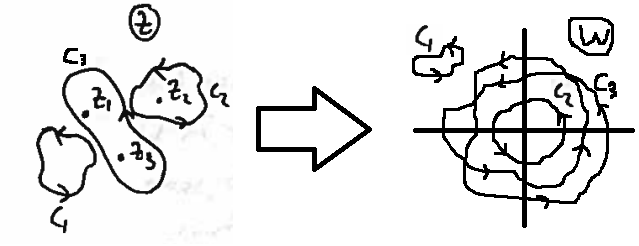
\includegraphics[width=\linewidth]{complex/argthm}
	\captionsetup{font=small} 	
\end{figure}
\noindent Another statement of the argument theorem is that along the path, $C$, the argument of $w$ changes by $2n\pi$ if $n$ zeroes are enclosed by $C$.
 If $C$ encloses 1 zero then $C$ wraps around $w=0$ once and therefore the argument of $w$ increases by $2\pi$ around the contour.
%
\begin{examples}
	\begin{enumerate}
		\item Sketch the curves or regions
		\begin{enumerate}
			\item $|z-1|=2$
			\item $Re[e^z]=1$ for $\frac{-\pi}{2} < y < \frac{\pi}{2}$
			\item $|z-1|<|z+1|$
		\end{enumerate}
		\item Verify the following identities:
		\begin{enumerate}
			\item $\sinh(iz)=i\sin(z)$
			\item $\arcsin(iz)=i$arcsinh$(z)$
		\end{enumerate}
		\item Sketch the mapping of $f(z)=e^z$, like in the example above.
		
		 [hint: $e^z=e^{x+iy}=e^xe^{iy}$]
	\end{enumerate}
\end{examples}
%
%
%
\section{Differentiation}
\subsection{Cauchy-Reimann conditions}
The problem with functions of a complex variable is that they may not be differentiable!
 But how do we know if a function is differentiable? 
 We can conclude that the differential of a function must be independent of direction.
 Lets start with the definition of a derivative, which should be familiar.
%
\begin{equation*}
\frac{\diff f}{\diff z}=\lim_{\delta z\to 0}\frac{f(z+\delta z)-f(z)}{\delta z}
\end{equation*}
%
Suppose that $\delta z=\delta x + i\delta y$.
 Then the derivative should be the same regardless of whether we set $\delta y=0$ and then approach the limit in the x-direction, or if we set $\delta x=0$ and approach the limit from the y-direction.
 If they give different answers, then the limit doesn't exist; if the limit does exist then the function is called analytic.
\par 
Note that rather than using X and Y to denote the real and imaginary parts of $f(z)$ we often use $u$ and $v$ to avoid confusion.
 Now we will find the criteria that a function must satisfy in order to be analytic.
 First we take a Taylor expansion of $f(z)$ to obtain
%
\begin{equation}
	 \label{eq:totaldcmplxv}
	 \delta f=\delta x \left(\frac{\partial u}{\partial x} + i \frac{\partial v}{\partial x}\right) + \delta y \left(\frac{\partial u}{\partial y}+i\frac{\partial v}{\partial y}\right) + O\left({\delta x}^2,{\delta y}^2\right)
\end{equation}
%
 which we will use to derive the \emph{Cauchy-Reimann} conditions for an analytic function.
 If we use the definition of the derivative and set $\delta y=0$ in equation \ref{eq:totaldcmplxv} we can show:
%
\begin{equation*}
	\frac{\diff f}{\diff z}=\lim_{\delta x\to 0}\left(\frac{\partial u}{\partial x} + i \frac{\partial v}{\partial x}\right) + O(\delta x).
\end{equation*}
%
Similarly, for $\delta x=0$, and recalling that we are taking the limit $i\delta y \rightarrow 0$, we can show that
%
\begin{equation*}
\frac{\diff f}{\diff z}=\lim_{\delta y\to 0}\frac{1}{i}\left(\frac{\partial u}{\partial y} + i \frac{\partial v}{\partial y}\right) + O(\delta y).
\end{equation*}
%
Requiring that these expressions are equal to each other, and remembering that $1/i=-i$, we obtain the Cauchy-Reimann conditions
%
\begin{equation}
	\frac{\partial u}{\partial x}=\frac{\partial v}{\partial y},
\end{equation}
%
\begin{equation*}
	\frac{\partial v}{\partial x}=-\frac{\partial u}{\partial y}, 
\end{equation*}
%
which if satisfied, implies $f(z)$ is analytic.
 Being more rigorous\footnote{I think it comes from the fact that we proved it for 2 orthogonal directions in a 2 dimensional plane so that covers all directions, but I am not sure.}, we would need to prove that satisfying these conditions implies that the limit is the same from all directions and vice versa, but we do not require that level of depth. 
 It should be noted that L'Hopital's rule, the chain rule, and the product rule still work for complex variables.
%
%
\begin{examples}
	Show that, given $f(z)=u+iv$ is analytic:
	\begin{enumerate}
		\item $\nabla^2u=\nabla^2v=0$
		\item $\pmb{\nabla} u \cdot \pmb{\nabla} v=0$
		\item $f(z)$ must be a function of $z$ and not $\overline{z}$
		
		[Hint: write $x=(z+\overline{z})/2$ and $y=(z-\overline{z})/2$ and show $\partial f/\partial \overline{z}=0$ and $\partial f/\partial z=\diff f/\diff z$]
	\end{enumerate}
\end{examples}
\subsubsection{solutions}
\begin{enumerate}
	\item This one is relatively simple, just write:
	\begin{equation*}
	\nabla^2u=\frac{\partial}{\partial x}\left(\frac{\partial u}{\partial x}\right)+\frac{\partial}{\partial y}\left(\frac{\partial u}{\partial y}\right)
	\end{equation*}
	and sub in the Cauchy-Reimann conditions to get
	\begin{equation*}
	\nabla^2u=\frac{\partial^2v}{\partial y \partial x}-\frac{\partial^2v}{\partial x \partial y}
	\end{equation*}
	%
	which equals zero by the commutative property of differentials. The same approach can be taken for $v$. functions that satisfy this equation, 'Laplace's equation' are called harmonic functions, this property of analytic functions will be useful later.
	%
	%
	\item Showing this will also be important for the next section. First write out the vectors
	\begin{equation*}
	\pmb{\nabla}u=\left(\frac{\partial u}{\partial x},\frac{\partial u}{\partial y}\right)~~\&~~\pmb{\nabla}v=\left(\frac{\partial v}{\partial x},\frac{\partial v}{\partial y}\right),
	\end{equation*}
	then using the Cauchy-Reimann conditions that indentity is easy to show.	
	 In the example mapping above and the problem you may have notices that your lines of constant x and lines of constant y appear to cross at right angles, this proves that is true for any region in which the function is analytic.
	%
	%
	\item This needs the Cauchy-Reimann conditions again
	$$\frac{\partial f}{\partial \overline{z}}=\left(\frac{\partial u}{\partial x}+i\frac{\partial v}{\partial x}\right)\frac{\partial x}{\partial \overline{z}}+\left(\frac{\partial u}{\partial y}+i\frac{\partial v}{\partial y}\right)\frac{\partial y}{\partial \overline{z}}     $$
	Then using $\partial x/\partial \overline{z}=1/2$ and $\partial y/\partial \overline{z}=i/2$ and the Cauchy Reimann conditions we can show $\partial f/\partial \overline{z}=0$. For the second part, use the same procedure to show
	\begin{equation*}
	\frac{\partial f}{\partial z}=\left(\frac{\partial u}{\partial x} + i \frac{\partial v}{\partial x}\right)=\frac{1}{i}\left(\frac{\partial u}{\partial y} + i \frac{\partial v}{\partial y}\right)=\frac{\diff f}{\diff z}.
	\end{equation*}
\end{enumerate}
%
%
\section{Conformal Mappings}
 